\documentclass[12pt,journal,draftclsnofoot,onecolumn]{IEEEtran}
\usepackage[T1]{fontenc}
\usepackage[utf8]{inputenc}
\usepackage{times}
\usepackage{amsmath,amssymb}
\usepackage{graphicx,booktabs,array,tabularx}
\usepackage{tikz}
\usepackage{setspace}
\usepackage[mathlines]{lineno}
\usepackage{url}
\usepackage[hidelinks]{hyperref}
\usetikzlibrary{arrows.meta,positioning}
\graphicspath{{figures/}}
\newcommand{\code}[1]{\texttt{\detokenize{#1}}}
\newcommand{\roundeven}{\operatorname{round}_{\mathrm{even}}}
% Generated by scripts/generate_paper_evidence.py; do not edit.
% research/evidence/audit.json SHA256: b606425695b69a625f5a0a3e9b9584958e9dc4bbe4b68301bac47f06c63b479e
% research/evidence/grouped-split-v1.json SHA256: bd919da4a91c40cecf95ccec211fec1bae2e55e587a7faa7f81ac140e6bd347f
% Counts describe recorded artifacts, not independent or clinical validity.
% AuditDuplicate* uses oriented-RGB exact-pixel groups; percentages omit the percent sign.
% CandidateRepeatedPixels counts excess eligible records above unique pixels.
\newcommand{\AuditClasses}{72}
\newcommand{\AuditImages}{48,693}
\newcommand{\AuditTrainImages}{36,852}
\newcommand{\AuditTrainInstances}{56,287}
\newcommand{\AuditValidImages}{5,922}
\newcommand{\AuditValidInstances}{8,805}
\newcommand{\AuditTestImages}{5,919}
\newcommand{\AuditTestInstances}{8,868}
\newcommand{\AuditFlaggedImages}{65}
\newcommand{\AuditDuplicateGroups}{138}
\newcommand{\AuditDuplicateImages}{276}
\newcommand{\AuditTrainValidGroups}{63}
\newcommand{\AuditTrainTestGroups}{56}
\newcommand{\AuditValidTestGroups}{19}
\newcommand{\NutritionRows}{1,010}
\newcommand{\MappingRows}{103}
\newcommand{\CoverageExact}{19}
\newcommand{\CoverageExactPercent}{26.39}
\newcommand{\CoverageAutomatic}{55}
\newcommand{\CoverageAutomaticPercent}{76.39}
\newcommand{\CoverageCurrent}{72}
\newcommand{\CoverageCurrentPercent}{100.00}
\newcommand{\MappingReviewCount}{21}
\newcommand{\CandidateSourceImages}{40,797}
\newcommand{\CandidateGroups}{23,933}
\newcommand{\CandidateQuarantinedImages}{11,002}
\newcommand{\CandidateQuarantinedGroups}{9,274}
\newcommand{\CandidateTrainImages}{26,384}
\newcommand{\CandidateTrainGroups}{10,251}
\newcommand{\CandidateTrainUniquePixels}{26,251}
\newcommand{\CandidateValidImages}{5,655}
\newcommand{\CandidateValidGroups}{2,203}
\newcommand{\CandidateValidUniquePixels}{5,629}
\newcommand{\CandidateTestImages}{5,652}
\newcommand{\CandidateTestGroups}{2,205}
\newcommand{\CandidateTestUniquePixels}{5,620}
\newcommand{\CandidateOldOverlapGroups}{5,548}
\newcommand{\CandidateEligibleImages}{37,691}
\newcommand{\CandidateRepeatedPixels}{191}
\newcommand{\CandidateUnresolvedImages}{9,127}
\newcommand{\CandidateConflictImages}{1,455}
\newcommand{\CandidateIssueGroupImages}{542}
\newcommand{\CandidateEmptyGroupImages}{424}

\onehalfspacing\setlength{\emergencystretch}{3em}

\begin{document}
\title{AI-Based Food Recognition with Nutrition-Aware Recommendations:\\A System and Reproducibility Audit}
\author{Jaspreet~Singh and Inderpal~Singh%
\thanks{Department of Computer Science and Engineering, National Institute of Technology Srinagar, Kashmir 190006, India. Draft author details are subject to confirmation before external submission.}}
\markboth{Supervisor Review Draft -- September 2026}{Singh and Singh: Food Recognition and Reproducibility Audit}
\maketitle

\begin{abstract}
An image-based food diary must distinguish a detected label, a database nutrient estimate, an assumed portion, and recorded consumption. This paper presents an educational Indian-food application and audits the evidence supporting it. The system combines YOLO11s detection, per-100-g nutrition lookup, user-estimated gram portions, an explicitly saved browser journal, and context-labeled advice. A read-only census of \AuditImages{} exported images across \AuditClasses{} classes identifies \AuditDuplicateGroups{} exact-duplicate groups spanning the archived partitions and malformed annotation records in \AuditFlaggedImages{} images. Source-byte matching and within-export filename-family grouping connect \CandidateOldOverlapGroups{} candidate groups across those partitions. A review-only reassignment retains class representation while quarantining \CandidateQuarantinedImages{} records; it does not establish independent test data for the existing checkpoint. Nutrition lookup is available for \CoverageExact{}/\AuditClasses{} classes under normalized exact matching, \CoverageAutomatic{}/\AuditClasses{} without precomputed mappings, and \CoverageCurrent{}/\AuditClasses{} with the current mapping layer. These are availability counts, not correctness estimates. The study contributes an inspectable system description, fingerprinted audit artifacts, and a concrete recovery protocol. It does not establish a novel detector, improved logging behavior, measured food mass, or medical efficacy. Independent detector evaluation, qualified mapping review, and asset-permission decisions remain necessary before broader claims.
\end{abstract}
\begin{IEEEkeywords}
Food recognition, nutrition databases, data leakage, reproducibility, software verification.
\end{IEEEkeywords}

\section*{Purpose of this review copy}
This manuscript is prepared for supervisor feedback, not external submission. It reports completed software and audit work separately from historical observations and proposed experiments. The author list, rights statements, study scope, and next evaluation protocol require confirmation. The companion conference-style draft is a shorter presentation of the same study, not a separate experiment.
\linenumbers
\modulolinenumbers[5]

\section{Introduction}
A food-diary interface needs more than the name of an object in a photograph. It must specify which nutrient record is attached to that label, the quantity used in the calculation, whether the user accepts the detection, and whether the meal was actually recorded as consumed. A plausible-looking calorie total can be wrong even when the underlying arithmetic is correct. Detection errors, recipe mismatch, portion assumptions, and generated advice therefore require different evidence.

This distinction is important for the Indian-food vocabulary used here. Labels such as \code{rice}, \code{palak_paneer}, and \code{chicken_biryani} are not ingredient measurements. Regional names can overlap, and one visual label may encompass several preparations. A match to a named database recipe is an implementation choice; a matching name alone does not establish nutrient equivalence with the photographed dish.

We study the existing \emph{AI-Based Food Recognition with Nutrition-Aware Recommendations} application as an engineering case study. The detector, nutrition database, matching rules, and health-context policy were preserved during this review. Rather than propose another model, we examine the relationship between the implemented system and the claims supported by its artifacts. This is motivated by the broader distinction between reporting a working machine-learning pipeline and establishing that its evaluation is independent \cite{kapoor2023leakage}.

The study addresses four questions:
\begin{enumerate}
\item RQ1: Which observable identity, partition-overlap, and annotation problems occur in the archived merged export?
\item RQ2: What does candidate source-family reconstruction establish about a new partition, and which relationships remain unresolved?
\item RQ3: How does lookup availability differ between normalized exact matching, automatic lookup, and the current precomputed mapping layer?
\item RQ4: Which application invariants are implemented and tested, and which nutrition, advice, and usability claims remain unvalidated?
\end{enumerate}
The contributions are a contract-accurate system description, a full-export audit with source-lineage recovery tooling, and a measured availability comparison with an explicit independent-review protocol. The results do not establish architectural priority over prior integrated systems or clinical validity.

\section{Related Work}
Food computing encompasses recognition, retrieval, recommendation, and monitoring rather than a single visual task \cite{min2019food}. Im2Calories already connected image analysis with a food diary and nutritional estimation \cite{meyers2015im2calories}. Consequently, recognition followed by nutrition lookup is not claimed as a new pipeline in this work.

IndianFoodNet studied detection of Indian foods using deep-learning models \cite{indianfoodnet_2023}. More recent Indian Thali work integrates multi-dish segmentation and recognition with weight and nutrition estimation \cite{indian_thali_2025}. These studies support the relevance of regional, multi-item analysis, but their datasets and evaluation protocols differ from the merged export examined here. Their performance numbers are not used as baselines for this checkpoint.

Nutrition5k supplies component-weight and nutrition references for food analysis \cite{thames2021nutrition5k}. That supervision differs fundamentally from multiplying database values by user-entered grams. Without measured quantities and an independently established recipe reference, the present application's totals are estimates based on selected assumptions, not validated image-derived nutrient measurements.

The Indian Nutrient Databank (INDB) provides the main food-composition resource used by the application \cite{development_indb_2024}. Its recipe calculations do not remove variation in ingredients, cooking yield, or preparation. The subsequent corrigendum corrects attribution to the source food-composition publications, not the application's mappings or nutrient estimates \cite{indb_corrigendum_2025}. Provenance and nutritional correctness must therefore be assessed separately.

Finally, evaluation leakage is not limited to identical filenames. Kapoor and Narayanan discuss non-independence and leakage in machine-learning-based science \cite{kapoor2023leakage}. Barz and Denzler use near-duplicate search and human review to study contamination beyond simple exact matching \cite{barz2020duplicates}. We use exact identities and explicit filename-family heuristics as auditable diagnostics, not as proof that every related image has been found. No effect size from another dataset is transferred to this detector.

A recent preprint on FKG.in separates structural, semantic, and source-fidelity checks for LLM-extracted Indian recipe knowledge \cite{gupta2026validatingfkg}. It reinforces the need to distinguish syntactic validity from supported food knowledge. Its knowledge-graph curation task differs from the present fixed-label database lookup, and its results are not a matched benchmark or clinical validation of this application.

\section{Application and Data Contracts}
\subsection{Scope and inference}
The application is configured to serve a static Next.js frontend and a FastAPI backend at one website address. Its production configuration uses native Python hosting and CPU inference. YOLO11s is an existing Ultralytics detector, cited as software rather than as a new architecture introduced here \cite{ultralytics2024}. The current production checkpoint contains \AuditClasses{} class names and occupies 19,211,162 bytes (approximately 18.32 MiB); this is not the Python bundle size or process memory.

The application's inference call uses image size 640, confidence threshold 0.25, and non-maximum-suppression intersection-over-union threshold 0.45. Retained boxes are returned in descending confidence order with pixel coordinates for the processed image. Legacy class-specific overrides use names that do not match the current lower-snake-case checkpoint labels; they do not raise thresholds for this checkpoint. Confidence scores are not calibrated probabilities of nutritional correctness. Application operating thresholds must also be distinguished from the archived evaluation settings described in Appendix~\ref{app:historical}.

The browser accepts source files up to 25 MiB and rejects decoded images exceeding 25 million pixels. It normalizes orientation, composites transparency on white, scales the longest side to at most 1,600 pixels, and attempts JPEG encoding at successively lower quality until the result is at most 3.8 MiB. The same processed file is uploaded and displayed. The backend independently accepts only supported JPEG, PNG, or WebP decoding, at most 4 MiB of uploaded bytes, and at most 25 million decoded pixels. These controls support coordinate consistency and bounded inputs, not recognition accuracy.

\begin{figure}[tbp]
\centering
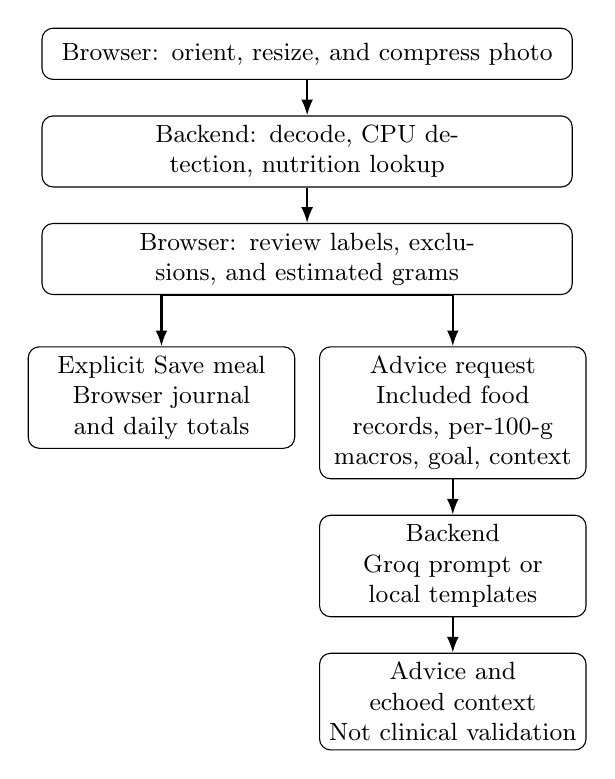
\begin{tikzpicture}[
 node distance=0.45cm,
 box/.style={draw,rounded corners,align=center,text width=6.5cm,minimum height=0.65cm,font=\small},
 side/.style={box,text width=3.15cm},
 arr/.style={-{Latex[length=2mm]},thick}]
\node[box] (upload) {Browser: orient, resize, and compress photo};
\node[box,below=of upload] (analysis) {Backend: decode, CPU detection, nutrition lookup};
\node[box,below=of analysis] (review) {Browser: review labels, exclusions, and estimated grams};
\node[side,below=0.65cm of review,xshift=-1.85cm] (save) {Explicit Save meal\\Browser journal and daily totals};
\node[side,below=0.65cm of review,xshift=1.85cm] (request) {Advice request\\Included food records, per-100-g macros, goal, context};
\node[side,below=of request] (provider) {Backend\\Groq prompt or local templates};
\node[side,below=of provider] (advice) {Advice and echoed context\\Not clinical validation};
\draw[arr] (upload)--(analysis);
\draw[arr] (analysis)--(review);
\draw[arr] (review.south)-|(save.north);
\draw[arr] (review.south)-|(request.north);
\draw[arr] (request)--(provider);
\draw[arr] (provider)--(advice);
\end{tikzpicture}
\caption{Separate recording and advice paths. Saving is not triggered by analysis. Selected grams and saved history do not enter the advice request; Groq receives only the name/energy subset of its food records.}
\label{fig:flow}
\end{figure}

\subsection{Nutrition lookup and its limitations}
The SQLite database contains \NutritionRows{} food rows and \MappingRows{} detector-to-row mappings, including legacy labels. All \AuditClasses{} current canonical classes have precomputed entries. The local INDB workbook is byte-identical to the authors' public artifact at the pinned revision recorded with the evidence \cite{indb_artifact_2024}. Five additional records use product or recipe sources for Bhakarwadi, Ghevar, Jalebi, Khandvi, and Nandu Kari \cite{fatsecret_bhakarwadi_2026,clearcals_ghevar_2026,clearcals_jalebi_2026,clearcals_khandvi_2026,clearcals_nandu_kari_2026}. These are source-attributed estimates, not measurements of the uploaded meal.

Offline construction prioritizes developer-defined class mappings. Otherwise, it calls a helper that compares normalized names and aliases, with an outer acceptance threshold of 0.78. Supplemental rows are inserted before mappings are constructed; they are not a separate inference branch. The helper is not an edit-distance or learned semantic matcher. It accepts normalized equality, or alias containment scored by a string-length ratio, with an internal minimum of 0.5.

Runtime first checks the precomputed mapping, then normalized equality, highest-ratio containment of at least 0.5, and the first alias-variation containment without a score gate. Its final helper call has an outer 0.4 threshold, but the helper does not return nonexact candidates below its own 0.5 minimum. Alias variations are constructed from a set, so ambiguous first-match fallbacks are not guaranteed to select the same row across processes. Current canonical precomputed mappings bypass that ambiguity. We therefore avoid describing the fallback as a deterministic, clinically conservative fuzzy matcher.

The API preserves source labels, optional source URLs, and mapping cautions. A missing lookup leaves the detection visible with unavailable nutrient values. Scores attached to precomputed mappings are heuristics; \MappingReviewCount{} current mappings score below 0.9 or lack a score. Neither a score of 1.0 nor complete macro fields demonstrate recipe equivalence. Repeated labels are deduplicated for lookup within an analysis, and a 256-entry per-instance cache avoids some repeated read-only database queries without merging the detections themselves.

\subsection{Portion estimates, missingness, and recorded consumption}
Let $I_m$ be the included detections in a meal draft $m$, and let $\mu(c)$ map a class to a database-row index or to $\bot$ when unavailable. Each row provides a per-100-g column vector $\mathbf{v}_r$ containing energy in kcal and protein, carbohydrate, and fat in grams. The known subset is
\begin{equation}
K_m=\{q\in I_m:\mu(c_q)\ne\bot\}.
\end{equation}
For user-estimated weight $w_q$, the known subtotal and incompleteness flag are
\begin{align}
\widehat{\mathbf{T}}_m^{\,known}
 &=\sum_{q\in K_m}\frac{w_q}{100}\mathbf{v}_{\mu(c_q)},\label{eq:portion}\\
u_m&=\mathbf{1}\{I_m\setminus K_m\ne\varnothing\}.\label{eq:missing}
\end{align}
No undefined missing-row vector is indexed, and unknown nutrients are not assumed to equal zero. Portions default to 100 g and can be changed from 25 to 1,000 g in 25 g steps. For example, 125 g multiplies each known per-100-g value by 1.25. Excluding an item removes it from both the subtotal and its missingness calculation.

Let $\mathcal{S}_d$ be explicitly saved meals whose stored local calendar date equals day $d$. Daily display uses
\begin{equation}
\widehat{\mathbf{T}}_d^{\,known}
=\sum_{m\in\mathcal{S}_d}\widehat{\mathbf{T}}_m^{\,known},
\qquad
u_d=\bigvee_{m\in\mathcal{S}_d}u_m.
\label{eq:day}
\end{equation}
An unsaved scan contributes nothing to $\mathcal{S}_d$. Saving updates by draft identity, so repeated clicks do not create additional meals; editing preserves the saved record's original timestamp and local date. Starting a new scan creates a new draft. The current day refreshes on focus, visibility changes, and local midnight. Displaying excess above a goal does not change the saved known subtotal.

Version-1 browser storage contains draft food names/labels (including excluded items), grams, inclusion flags, per-100-g values, source labels, timestamps, local dates, and goal/calorie preferences. It does not retain photos, health selections, bounding boxes, confidence, source URLs, or mapping notes. Thus the current journal is not a complete scientific provenance archive. Unsupported or corrupt storage is not silently overwritten; scanning remains available while saving is paused with an error.

\subsection{Goals and health-context advice}
Goal targets are separate from meal estimates. Existing policy supplies three positive base weights $b_k$ and condition modifiers $r_k$. With $k\in\{c,p,f\}$,
\begin{equation}
a_k=100\frac{b_kr_k}{\sum_j b_jr_j},\qquad
p_c=\roundeven(a_c),\quad
p_p=\roundeven(a_p),\quad p_f=100-p_c-p_p.
\end{equation}
For calorie target $E$, the implemented gram targets are
\begin{equation}
G_c=\roundeven(Ep_c/400),\quad
G_p=\roundeven(Ep_p/400),\quad
G_f=\roundeven(Ep_f/900).
\end{equation}
The frontend fallback reproduces Python's ties-to-even rounding. Stored endurance weights 55/20/20 sum to 95, not 100; with no condition modifier they produce rounded percentages 58/21/21. The backend accepts integer calorie targets from 1 to 5,000, whereas browser preferences allow 500 to 5,000; the validation records this boundary difference without changing the API. These values are documented as software policy, not clinically validated prescriptions. There are nine context options: no condition and eight named health contexts.

The recommendation endpoint receives up to ten included food records with per-100-g macro fields, a goal, and a session-only health context. The Groq prompt retains food names and rounded \emph{energy} per 100 g, not the protein, carbohydrate, or fat numbers. Neither the endpoint nor the prompt receives selected grams, target calories, consumed/remaining totals, or saved history. The prompt states that a scan does not establish consumption and that unsupplied nutrient quantities and medical suitability should not be inferred.

Production uses asynchronous Groq followed by local templates, with a 20-second provider timeout and automatic retries disabled. The local fallback uses the first two food names; condition templates take precedence over goal templates, and nutrient values do not select the advice. Some retained templates nevertheless use consumption-assuming or suitability language. Prompt constraints and fallback availability therefore do not establish safe or nutritionally appropriate advice.

A context change hides previous advice immediately. Superseded requests are aborted and late responses discarded. A successful response must echo the expected health key before the interface shows labels such as \emph{Adjusted for diabetes} or \emph{Adjusted for high blood pressure}; no-condition responses use \emph{General nutrition guidance}. The echoed key is an application consistency check, not evidence that an expert evaluated the advice.

\section{Audit Methods}
\subsection{Artifacts and unit of analysis}
The audit examines the archived \AuditClasses{}-class export, five locally available source downloads, the nutrition database, and recorded training/evaluation artifacts. It does not retrain the detector, repair labels, overwrite the export, or create nutritional ground truth. The image census concerns exported file records; these are not necessarily distinct original photographs.

\begin{table}[tbp]
\centering
\caption{Locally indexed source exports. Class counts are source entries, not a summed distinct vocabulary. Versions and URLs come from local export metadata.}
\label{tab:sources}
\begin{tabular}{lrr}
\toprule
Export & Listed classes & Images\\
\midrule
Indian food detection v1 \cite{source_project_z0tql} & 17 & 9,053\\
Indian food v6 \cite{source_microplastics} & 29 & 8,406\\
IndianFood-7 v2 \cite{source_indianfood7} & 7 & 1,949\\
IndianFoodNet v1 \cite{source_indianfoodnet} & 30 & 13,036\\
South Indian food detection v19 \cite{source_south_indian} & 31 & 8,353\\
\midrule
Total & --- & \CandidateSourceImages\\
\bottomrule
\end{tabular}
\end{table}

The historical builder pools source partitions, canonicalizes labels, splits sample indices, and adds further training-only augmentation. Its 70/15/15 target was not the final export proportion after augmentation. Several downloads already contained augmented variants. A new sample-index split cannot undo those source relationships.

\subsection{Exact identities and annotation checks}
For each exported image, the audit records file path, split, SHA-256 of file bytes, label-file hash, accepted class indices, dimensions, and validation flags. A second image identity hashes the EXIF-oriented RGB dimensions and pixel bytes, without resizing. Byte and pixel groups are each counted as crossing partitions when their members occupy more than one split. Pair-specific counts are counts of groups, not all Cartesian pairs of files. Cryptographic equality establishes the compared identity only; it cannot exclude near-duplicate crops or different transforms.

A nonblank YOLO annotation row must contain exactly five fields, an integer class in range, finite coordinates, centers in $[0,1]$, and width/height in $(0,1]$. Accepted-instance counts omit rejected rows. These checks do not verify that box edges stay in frame, all visible foods are annotated, classes are semantically correct, or boxes correspond to distinct objects. Empty accepted labels caused by malformed rows are not treated as verified negative images.

\subsection{Candidate lineage and quarantine}
The recovery tool first rereads exported images and labels against the saved manifest, rejecting stale membership, hashes, or class ordering. Source records are indexed by byte SHA-256 and filename-family key; source images do not undergo the exported-image pixel-hash pass. A family key is the within-export filename prefix before the earliest \code{.rf.<32 hex digits>} marker. Generic names in different exports are not joined by name alone.

A union-find graph joins equal bytes, equal exported pixel identities, and common source-family keys. Source-only records participate so that identical source copies can connect two families transitively. A connected component containing exported images becomes a candidate grouping unit. This is an explicit linkage heuristic, not a manually verified original-photo identifier: it can both merge unrelated generic names within a source and miss related images with different names.

An entire component is quarantined if lineage is unresolved, a source naming pattern is unrecognized, any exported member has a decode/annotation flag or no accepted annotations, or equal exported pixels have different label-file hashes. Byte inequality alone cannot distinguish formatting from numeric changes; the follow-up finds none of the direct conflicts to be formatting/order-only. Quarantine means an unassigned manifest status; files are not removed.

\subsection{Candidate partition assignment}
Eligible components are assigned as indivisible units. The tool orders them by rarity of represented classes, decreasing component size, and seeded SHA-256 tie-breaking. A greedy rule minimizes the change in normalized squared deviations from target image totals and per-class \emph{image} counts. The seed is 42, and target ratios are 0.70/0.15/0.15 over eligible records. This is a balancing heuristic, not a globally optimal stratifier or an object-instance balancing method.

If $\mathcal{G}_{tr},\mathcal{G}_{va},\mathcal{G}_{te}$ are sets of eligible component identifiers, the checked invariant is pairwise disjointness:
\begin{equation}
\mathcal{G}_s\cap\mathcal{G}_t=\varnothing\quad\text{for every }s\ne t.
\end{equation}
Known byte/pixel identities and family keys must not occur in separate components. This invariant is established by construction and validation; it does not show that all real-world related photographs have been discovered. The existing checkpoint has already been developed with the old export, so reassignment alone cannot produce its independent test set.

\subsection{Lookup availability comparison}
The comparison uses the fixed current database and all \AuditClasses{} canonical labels, without measuring detections. Three methods are evaluated: normalized exact matching; the existing automatic runtime lookup after clearing precomputed mappings in an isolated service instance; and the current service with those mappings retained. For method $j$,
\begin{equation}
A_j=\frac{1}{|\mathcal C|}\sum_{c\in\mathcal C}\mathbf{1}\{\mu_j(c)\ne\bot\}.
\label{eq:coverage}
\end{equation}
The database remains read-only. The automatic method is an alias/containment pipeline, not an independently tuned retrieval baseline. The earlier availability run did not record its hash seed; the follow-up separately records eight fixed seeds and confirms order-sensitive ambiguous selections.

The metric asks only whether a row was returned. It does not assess correctness, uncertainty calibration, ingredient equivalence, nutrient error, or clinical advice. No supplemental-removal or macro-verification-removal experiment was conducted, and no such result is claimed.

\subsection{Software verification}
Backend unit/contract tests, frontend arithmetic and transport tests, and mocked browser workflows examine the invariants in Table~\ref{tab:software}. The application pipeline includes lint, type checks, generated-contract drift checks, production frontend build, and tests without provider credentials. Research-tool tests use synthetic images/records. Operational website checks and archival detector evaluation are different evidence categories; neither is a clinical or user study.

\begin{table}[tbp]
\centering
\caption{Software properties covered by tests, not estimates of health or usability benefit.}
\label{tab:software}
\begin{tabularx}{\linewidth}{@{}p{0.23\linewidth}X@{}}
\toprule
Area & Test scope\\
\midrule
Arithmetic/journal & Gram scaling, exclusions, missingness, save/update identity, edits, deletion/undo, reload, midnight and storage failure\\
Advice state & Context changes during requests, stale/mismatched responses, source labels, timeout/fallback, retries initiated by the user\\
Upload/API & Orientation/processed-image alignment, invalid and oversized inputs, rate/busy responses, no detections, request timeouts\\
Interface & Desktop and 360-pixel layout, keyboard upload/reset, visible errors and accessible status messages\\
Backend resources & Lifecycle cleanup, dependency overrides, provider saturation, and operational-log field restrictions\\
\bottomrule
\end{tabularx}
\end{table}

\section{Results}
\subsection{RQ1: Archived export audit}
The census contains \AuditImages{} records. Table~\ref{tab:export} separates file counts, accepted annotation instances, and images with rejected rows. The archived evaluator reported 8,812 validation and 8,875 test instances; the strict audit accepts seven fewer rows in each. These are different counting procedures, not silently interchangeable ground-truth totals.

\begin{table}[tbp]
\centering
\caption{Original export census. Flagged-image counts are not inferred rates of semantic annotation error.}
\label{tab:export}
\begin{tabular}{lrrr}
\toprule
Partition & Images & Accepted instances & Flagged images\\
\midrule
Train & \AuditTrainImages & \AuditTrainInstances & 51\\
Validation & \AuditValidImages & \AuditValidInstances & 7\\
Test & \AuditTestImages & \AuditTestInstances & 7\\
\bottomrule
\end{tabular}
\end{table}

Both byte and oriented-pixel checks find \AuditDuplicateGroups{} cross-partition groups affecting \AuditDuplicateImages{} records: \AuditTrainValidGroups{} train--validation, \AuditTrainTestGroups{} train--test, and \AuditValidTestGroups{} validation--test groups. For example, the following test and training files have identical bytes:
\begin{quote}\small
\code{test0134-bhindi_masala.jpg}\\
\code{train16477-bhindi_masala.jpg}
\end{quote}
The amount of metric inflation cannot be inferred from the duplicate count. The audit also finds \AuditFlaggedImages{} flagged images, including zero-area boxes. It does not establish a semantic error rate or negative-image false-positive performance.

\subsection{RQ2: Candidate grouped partition}
Recovery forms \CandidateGroups{} components containing exported records; \CandidateOldOverlapGroups{} candidate lineage groups span the old partitions. This broader result reflects byte links and heuristic filename ancestry, not thousands of independently confirmed duplicate originals.

Table~\ref{tab:candidate} shows the review-only assignment. Its three eligible partitions each retain all \AuditClasses{} labels. However, record counts overstate independent evidence when within-family variants remain; some classes have only 17 labeled records in a candidate validation/test partition. Class presence is not a sample-size justification.

\begin{table}[tbp]
\centering
\caption{Candidate assignment, not a newly validated benchmark. Unique pixels are counted within each eligible partition; repeats are retained within groups.}
\label{tab:candidate}
\begin{tabular}{lrrr}
\toprule
Status & Groups & Images & Unique pixels\\
\midrule
Train & \CandidateTrainGroups & \CandidateTrainImages & \CandidateTrainUniquePixels\\
Validation & \CandidateValidGroups & \CandidateValidImages & \CandidateValidUniquePixels\\
Test & \CandidateTestGroups & \CandidateTestImages & \CandidateTestUniquePixels\\
Quarantine & \CandidateQuarantinedGroups & \CandidateQuarantinedImages & ---\\
\bottomrule
\end{tabular}
\end{table}

There are \CandidateEligibleImages{} eligible records and \CandidateRepeatedPixels{} extra records beyond their distinct pixel identities. Whole-group quarantine affects \CandidateQuarantinedImages{} images. Nonexclusive reason counts are \CandidateUnresolvedImages{} for unresolved lineage, \CandidateConflictImages{} for equal pixels with different label-file bytes, \CandidateIssueGroupImages{} for an annotation/decode flag in the component, and \CandidateEmptyGroupImages{} for a member with no accepted annotations. These propagated counts are not counts of individually proven faulty annotations and must not be added together.

Two earlier full reads produced identical assignment and source-inventory hashes in the same environment. The second script added input/class validation and had a different script hash. This demonstrates same-environment output repeatability for those runs, not independent replication or stability across every platform. The reports retain fingerprints but do not capture the complete historical execution environment.

\subsection{RQ3: Lookup availability}
Table~\ref{tab:availability} reports the completed comparison. Current mappings increase the number of classes receiving a row; there is no independent reference set demonstrating that the additional rows are correct. The \MappingReviewCount{} heuristic review flags remain useful for inspection but do not bound errors among the other mappings.

\begin{table}[tbp]
\centering
\caption{Availability over the fixed \AuditClasses{}-label vocabulary. These percentages are not mapping or nutrition accuracy.}
\label{tab:availability}
\begin{tabular}{lrr}
\toprule
Method & Classes with a row & Availability\\
\midrule
Normalized exact & \CoverageExact/\AuditClasses & \CoverageExactPercent\%\\
Automatic, no precomputed mappings & \CoverageAutomatic/\AuditClasses & \CoverageAutomaticPercent\%\\
Current mapping layer & \CoverageCurrent/\AuditClasses & \CoverageCurrentPercent\%\\
\bottomrule
\end{tabular}
\end{table}

The counts are a census of the selected vocabulary, not a random-sample estimate of performance on unseen foods; statistical confidence intervals would not turn them into correctness measurements. The workbook byte-identity comparison and supplemental source-value checks establish provenance/transcription consistency only.

\subsection{RQ4: Application verification}
The recorded source-revision checks passed backend, frontend, and mocked browser workflows, including saved-only daily totals and health-context response matching. The test coverage is specified in Table~\ref{tab:software}, not summarized as a medical-safety score. Tests verify that generated advice does not overwrite arithmetic; they do not verify every recommendation's content or prove lower hallucination frequency.

One executor worker runs inference, allowing one additional waiting analysis. The backend wait budget is 110 seconds and the browser analysis budget is 120 seconds; a timeout does not terminate a running worker. Recommendation capacity admits at most two concurrent operations without a waiting queue. Default rate limits are ten analysis and five recommendation requests per minute, keyed by remote address in an instance-local limiter. These are operational protections, not global spending controls or an availability guarantee.

\subsection{Validation follow-up}
A separate, fingerprinted review pass preserved the uncommitted manuscripts and inspected implementation before testing. Its reports record commands, environments, input identities and unsuccessful attempts as well as passing checks. The validation runs on Windows with Python 3.12.7; it is not a new verification of the locked Linux deployment or a new detector experiment.

Fresh full-export and grouping runs reproduced the earlier census, duplicate counts, dataset fingerprint, source inventory and candidate assignment hash. A separate annotation reader agreed on all 48,693 records. The 65 strict flags comprise 45 zero-width and 20 zero-height rows; 47 affected images have no accepted instances. All 65 originals and flagged records received an AI-assisted visual/numeric inspection, not qualified annotation approval. Among 104 identical-pixel groups with different label files (209 images), 69 differ in boxes with the same class multiset and 35 differ in class or instance multiplicity; none is explained solely by formatting/order. An additional edge-geometry check flagged 3,794 rows in 3,346 images at a $10^{-6}$ tolerance. These are review candidates, not automatically invalid annotations, and originals remain unchanged.

The smallest class-specific candidate-group counts are 43/9/11 in train/validation/test, which illustrates why image counts overstate independent support. A bounded perceptual screen sampled 2,020 records and compared 1,360,132 eligible cross-candidate-partition pairs, yielding 16 candidates at Hamming distance at most six. These pairs are queued for human review, not confirmed shared ancestors. Synthetic probes used 12 originals for each transform: all 12 were detected separately for JPEG compression and resizing, but none for cropping, mirroring or rotation. This screen cannot certify transformation independence or approve the candidate benchmark.

Independent workbook reconciliation found 1,014 source rows, nine duplicate-normalized-name omissions, 1,005 retained rows and five supplemental rows, yielding the existing 1,010-row database. All 4,040 nutrient-field comparisons agreed within an absolute tolerance of $10^{-9}$. The supplemental literals were also checked against their attributed per-100-g source records, with cached retrieval distinguished from successful direct access. This establishes transcription consistency, not photographed-recipe equivalence.

Separate rational-arithmetic oracles checked 162,036 goal/context/calorie combinations in each of the backend and frontend, covering every integer target from 500 to 5,000 across four goals and nine contexts. They found no discrepancies. The actual frontend additionally passed 2,880 class/portion cases, with 11,520 nutrient-field comparisons and maximum absolute floating-point deviation below $10^{-12}$. These results validate the implemented calculations at the declared tolerances, not the clinical basis of the policy.

Eight fixed hash seeds were tested over 181 food-label inputs for each of two lookup modes. Thirty method/label pairs returned different rows across seeds; six involved canonical labels only after precomputed mappings were removed. All current canonical mappings remained stable in these runs. The result confirms a bounded reproducibility concern in fallback lookup, not an independently measured wrong-match rate.

The offline recommendation matrix covered 216 goal/context/scenario combinations, and 16 SDK/mock-transport cases checked provider behavior without network calls. Extended browser tests covered all 36 goal/context combinations and delivered out-of-order responses for context, goal, included-food and scan changes. Two failed browser-harness attempts were retained and diagnosed before the corrected harness passed. Fallback text still requires qualified content review, and none of these checks demonstrates clinical safety.

\section{Interpretation and Threats to Validity}
The strongest supported finding is not a detector accuracy improvement but a mismatch between the independence assumed by older presentation and the identities found in its data. Grouping known relations and reporting quarantine makes that mismatch explicit. It does not quantify historical score inflation or complete the dataset repair.

Internal-validity threats include missed cross-source near duplicates, mistaken filename-family merges, unresolved broader family-level annotation differences, and incomplete lineage for locally augmented records. The direct identical-pixel label conflicts checked above are not merely formatting differences; their semantic resolution is still pending. No absence of exact overlap can certify independence. Valid empty negative examples are not established by this export. A reviewed original/representative policy is needed before interpreting a candidate partition as a benchmark.

Construct-validity threats arise from conflating class recognition, recipe equivalence, portion correctness, and health appropriateness. User-entered grams are assumptions; a database's presence is not a measurement of the meal; an echoed health key is not a clinical endorsement. Local templates can still imply consumption or suitability, and recommendations have no measured sodium, sugar, or ingredient quantities. The current application should remain an educational demonstration.

External-validity threats include the fixed 72-label vocabulary, source-specific capture and augmentation, limited independent support for some classes, and untested camera, lighting, and preparation distributions. Browser tests exercise designed scenarios, not representative users. The study does not show reduced logging effort, sustained adoption, improved diet, or medically safe personalization.

Reproducibility also has limits. Tools and aggregate evidence are present in the inspected checkout, but current public access was not verified; large full manifests are local artifacts and source access depends on provider permissions. Archived notebook outputs are not an immutable evaluation-time checkpoint record. Free hosting has quotas; release acceptance thresholds and a successful smoke test are not latency distributions, clinical validation, or service-level commitments.

\section{Prospective Evaluation for Supervisor Approval}
The following is proposed work, not completed evidence.

\subsection{Independent mapping assessment}
Freeze the database and candidate outputs before review. Define acceptable recipe equivalence, permitted approximations, unsupported labels, and genuinely ambiguous cases. Qualified reviewers should judge food-composition evidence without copying current outputs or heuristic scores. Preserve initial judgments and adjudicate disagreement.

The preserved version-1 template accepts a set $R_c$ of acceptable row names for each class. A nonempty prediction is a correct match if it belongs to $R_c$ and a wrong match otherwise. An abstention is correct when $R_c$ is empty and a missed supported case otherwise. A new version-2 packet separately represents indeterminate cases and preserves two initial reviews plus disagreement adjudication, tied to database and reference hashes. Indeterminate cases are reported separately and excluded from the scorable denominator; no judgments have been filled in. Report all four decision counts, not just coverage; add agreement and uncertainty appropriate to any sampling design. Format and attestation checks cannot establish actual expertise, blinding, or independence. The 72 current classes are a discovery set, not an untouched tuning benchmark.

\subsection{Independent detection and nutrition claims}
Review candidate group links, quarantine, representative selection, and annotations; freeze the resulting manifest before model selection. Retrain from an appropriate initialization on reviewed partitions or use a genuinely untouched external evaluation set. Document pretraining exposure and exact checkpoint hashes, packages, operating settings, selection rules, and dataset revision. Do not use the new partition to claim independent accuracy for the already-developed checkpoint.

Report per-class support and detection metrics, including background/no-food cases. Use uncertainty procedures that respect source-family dependence when making population claims. A baseline requires matched training data, budget, and evaluation settings; an augmentation ablation is needed only if an augmentation benefit is claimed. Nutrient-error claims additionally require independent recipe and portion references rather than guessed grams.

\subsection{Advice and user-facing benefit}
Evaluate recommendation content separately with qualified reviewers and a prespecified rubric for unsupported claims, context consistency, and appropriateness. Fix or explicitly delimit the inherited fallback wording before presenting it as consumption-aware advice. A usability or longitudinal study would need its own population, outcomes, consent, data handling, and institutional-review assessment. No such study or ethics approval is claimed here.

\section{Conclusion}
This work documents an Indian-food web application and audits its supporting evidence. The full export contains \AuditDuplicateGroups{} exact cross-partition groups and \AuditFlaggedImages{} images with strict annotation flags. Candidate lineage grouping exposes potential broader source relationships and produces a review-only partition with explicit quarantine. Current nutrition lookup covers all \AuditClasses{} labels, but that coverage does not demonstrate recipe or nutrient correctness. The practical contribution is a more inspectable separation of estimates, saved consumption, advice context, and evidence status. Independent evaluation and owner/supervisor approvals remain the next steps; additional interface features are not substitutes for those requirements.

\section*{Data, Code, and Review Artifacts}
The local audited checkout is identified by this repository reference, whose current public accessibility was not verified:
\href{https://github.com/jaspreet-jt-singh/Final_Year_Project/tree/0a4edfa92818945ccd7f16b023299c847c745f0d}{source revision 0a4edfa}.
Tracked reports under \code{research/evidence/} identify the model, database, workbook, scripts, and local manifest hashes. Numeric audit macros in this manuscript are generated from those reports and checked for drift. The new validation supplement accompanies this review copy; its uncommitted tooling and reports are not part of the linked base revision. Its baseline manifest records current-file hashes rather than treating the base commit as the identity of the revised papers.

Full manifests remain local in \path{.deployment/research/}. They are not automatically included in a repository checkout or this PDF. They must be packaged and supplied separately for artifact review when permissions allow. Source datasets should be obtained from their providers under applicable terms. Some source README files qualify crawled-image permissions despite an export-level CC BY label. Workbook identity is verified, but dataset, model, database, and figure redistribution permissions remain separate owner decisions. No new license or unrestricted asset release is asserted.

\section*{Draft Transparency and Author Confirmation}
AI-assisted tools supported code inspection, reference checking, and editorial revision of this draft. The authors must verify the resulting text, references, and analyses and take responsibility for the final manuscript. Authorship, contributions, correspondence details, funding, competing interests, acknowledgments, and any institutional-review requirements remain to be confirmed before an external submission. No new clinical experiment, participant study, detector training, or paper submission was performed during this review.

\appendices
\section{Historical Detector Evidence, Not an Independent Benchmark}
\label{app:historical}
The outputs in \code{notebooks/final_version_training.ipynb}, cells 8 and 9 in one-based file order, record validation and test evaluation of an exported \code{best.pt} path. Table~\ref{tab:historical} retains rounded historical values; it is not a new run or a clean held-out performance claim.

\begin{table}[tbp]
\centering
\caption{Archived notebook observations on overlapping partitions. Precision/recall were console-rounded; mAP values are rounded here to three decimals.}
\label{tab:historical}
\begin{tabular}{lrrrr}
\toprule
Partition & Precision & Recall & mAP$_{50}$ & mAP$_{50:95}$\\
\midrule
Validation & 0.847 & 0.807 & 0.830 & 0.692\\
Test & 0.842 & 0.801 & 0.820 & 0.680\\
\bottomrule
\end{tabular}
\end{table}

The notebook reports Ultralytics 8.4.60, Python 3.12.13, Torch 2.10.0+cu128, and a Tesla T4 with 14,913 MiB. Evaluation specifies data, device, and split without explicit confidence or NMS overrides. Its approximately 11 ms/image GPU inference timing excludes the deployed CPU/application path. It must not be presented as website latency or as a matched test of the application's 0.25/0.45 operating thresholds.

The merged training CSV has 100 distinct epochs. Its maximum logged validation mAP$_{50}$ is 0.83379 at epoch 78, whereas the maximum mAP$_{50:95}$ is 0.69226 at epoch 97. Neither fact proves which serialized checkpoint was selected. The current deployed and archived final checkpoint files have matching hashes, but the notebook did not record the evaluated checkpoint hash at runtime. A different notebook, \code{result-merge.ipynb}, evaluates an older checkpoint and is not the source of Table~\ref{tab:historical}.

Reconstruction of the two stage CSVs, covering epochs 1--55 and 56--100, agrees with the merged numerical cells. The time column resets on resumption; its final value is not total 100-epoch training time. The initial-training notebook contains a legacy 30-class workflow and cannot supply missing execution provenance for the archived 72-class initial stage. Available older-checkpoint prediction files cannot be used to independently recompute the final model's AP.

\section{Implementation Snapshot and Artifact Identity}
The production source uses Python 3.12, CPU Torch 2.6.0, Torchvision 0.21.0, headless Ultralytics 8.4.33, Next.js 16.3.4, and React 19.2.8. Model loading is lazy; startup health/readiness fields are operational status, not predictive quality. SQLite lookups use read-only connections. Uploads are not deliberately retained by application code, while hosting/provider handling remains subject to their own policies.

Table~\ref{tab:hashes} gives short identifiers for locating the full recorded fingerprints, not substitutes for the full hashes in the evidence files.
\begin{table}[tbp]
\centering
\caption{Artifact SHA-256 prefixes; full values are recorded in repository evidence.}
\label{tab:hashes}
\begin{tabular}{ll}
\toprule
Artifact & SHA-256 prefix\\
\midrule
Deployed checkpoint & \code{935a1b34365b}\\
Nutrition SQLite database & \code{3bdfb92fafd2}\\
Original INDB workbook & \code{65f91911de09}\\
Candidate assignments & \code{54fa9cc4cea5}\\
Historical final-training notebook & \code{9f927f3a2bba}\\
\bottomrule
\end{tabular}
\end{table}

\bibliographystyle{IEEEtran}
\bibliography{bibliography/references}
\end{document}
